\section{Limits}
\label{sec:limits}

\subsection*{Recommended Tutorials:}
\begin{itemize}[noitemsep]
	\item \nameref{chp:limits}, pg. \pageref{chp:limits}
\end{itemize}

\subsection*{Introduction:}

In this activity, students will use the \texttt{limit()}\index{limit} command to find various limits.

\subsection*{Exercises:}
\begin{enumerate}
    \item Calculate the limit $\displaystyle\lim_{x \to 1} \dfrac{\ln(x^4+1)-1}{x-2}$.
\marginnote[-0.5cm]{There is a shortcut for limits on the palettes toolbar under Calculus.\begin{center}
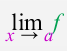
\includegraphics[scale=0.5]{tutorials/figures/palettelimit.png}
\end{center}}
    \item Plot the function 
    \[f(x)=\dfrac{|x|}{x}\] 
    over an appropriate range, and then use the \texttt{limit()}\index{limit} command to calculate the left-hand limit, the right-hand limit, and the two-sided limit as $x$ tends to zero.
    \marginnote[-1.8cm]{In Maple, the absolute value function $|\cdot|$ is denoted as \texttt{abs( )}.} \index{plot!discontinuities}
    \marginnote[-0.9cm]{Some versions of Maple may not properly display graphs of certain functions that contain discontinuities. In this case, include \texttt{discont=true} as a parameter in the \texttt{plot( )} command.}
    \item Consider the function $g(x)=\dfrac{x^2+x}{\sqrt{x^3+x^2}}.$
    \marginnote[0.1cm]{Use \texttt{sqrt()} to input a square root in Maple.}
			\begin{enumerate}
				\item Use the \texttt{plot()} command between $x=-2$ and $x=2$ to estimate the left-hand-limit, the right-hand limit, and the two-sided limit as $x$ tends to zero.
				\marginnote[0.1cm]{You need to find the limit as $x$ approaches zero, not as it approaches $-2$ or $2$.}
				\item Use the \texttt{limit()} command to verify your results from part (a).

			\end{enumerate}

    \item Estimate the value of 
    \[\displaystyle\lim_{t\to 0} \dfrac{\sin(t)}{\sin(\pi t)}\] 
    by using Maple's \texttt{plot()} command, and then check your answer with Maple's \texttt{limit()} command.
    	\marginnote[-1cm]{Do not forget to use \texttt{Pi} for $\pi$ and include multiplication between $\pi$ and $t$. You will also need to use $t$ instead of $x$ in your \texttt{plot()} command!}
		\item Calculate $\displaystyle\lim_{x \to \infty} \sqrt{x+1}-x$.\index{limit!at infinity}
    \marginnote[-0.2cm]{To denote $\infty$ in Maple, you need to type the word \texttt{infinity}.}
    \item Use the Limit Methods Tutor to explore the steps to calculate 
    \[\displaystyle\lim_{x \to -\infty} \sqrt{x^2+x+1}+x.\]\index{limit!at infinity}
    \marginnote[-1cm]{The Limit Methods Tutor is described on page \pageref{sec:limitmethodstutor}.}
    \index{limit!tutor}
\end{enumerate}